\chapter{Linear Programming}

\section{Introduction}

\subsection{Linear Programming}

Linear programming is a method to achieve the best outcome in a mathematical model whose requirements are represented by linear relationships. It is a special case of mathematical programming (mathematical optimization).

\begin{example}[Brewery]
    A brewery can invest its inventory of corn, hops and malt into producing some amount of ale and some amount of beer.  Per unit resource requirement and profit of the two items are as given below.

    \begin{table}[ht!]
        \centering
        \begin{tabular}{|c|c|c|c|c|}
            \hline
            Beverage      & Corn (pounds) & Hops (ounces) & Malt (pounds) & Profit (\$) \\ \hline
            Ale (barrel)  & 5             & 4             & 35            & 13          \\ \hline
            Beer (barrel) & 15            & 4             & 20            & 23          \\ \hline
            constraint    & 480           & 160           & 1190          &             \\ \hline
        \end{tabular}
    \end{table}

    Suppose it produces $A$ units of ale and $B$ units of beer. Then, we want to solve this program:
    \[
        \begin{matrix}
                        & \color{blue} \text{Ale} &   & \color{blue} \text{Beer} &      &      &                            \\
            \max        & 13A                     & + & 23B                      &      &      & \color{blue} \text{Profit} \\
            \text{s.t.} & 5A                      & + & 15B                      & \leq & 480  & \color{blue} \text{Corn}   \\
                        & 4A                      & + & 4B                       & \leq & 160  & \color{blue} \text{Hops}   \\
                        & 35A                     & + & 20B                      & \leq & 1190 & \color{blue} \text{Malt}   \\
                        & A                       & , & B                        & \geq & 0    &                            \\
        \end{matrix}
    \]
\end{example}

\begin{definition}[Linear Function]
    $f: \R^n \to \R$ is a \term{linear function} if $f(x) = a^Tx$ for some $a \in \R^n$. 
\end{definition}

\begin{example}
    For example, \[
        f(x_1, x_2) = 3x_1 - 5x_2 = \begin{pmatrix} 3 & -5 \end{pmatrix}^T \begin{pmatrix} x_1 \\ x_2 \end{pmatrix}
    \] We can see that $a$ is the vector of coefficients of the linear function.
\end{example}

\begin{itemize}
    \item \textbf{Linear objective}: $f$
    \item \textbf{Linear constraints}:
    \begin{itemize}
        \item $g(x) = c$, where $g: \R^n \to \R$ is a linear function and $c \in \R$
        \item Line in the plane (or a hyperplane in higher dimensions $\R^n$)
    \end{itemize}
\end{itemize}

Geometrically, $a$ is the normal vector of the line(or hyperplane) represented by $a^Tx = c$.

\begin{figure}[ht!]
    \centering
    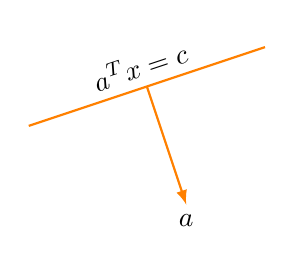
\begin{tikzpicture}[scale=0.5]
        \draw[thick,orange       ] (-3,-1) -- (3, 1) node[black,sloped,midway,above] {$a^Tx = c$};
        \draw[thick,orange,-latex] ( 0, 0) -- (1,-3) node[black,              below] {$a$};
    \end{tikzpicture}
\end{figure}

and $a^Tx \leq c$ is the \term{half-space} defined by the line.

\subsection{Finding the Optimal Solution}

\begin{example}
    Suppose we want to solve the following linear program: \[ \begin{matrix}
        \max        & x_1 & +    & 6x_2              \\
        \text{s.t.} & x_1 & \leq & 200               \\
                    & x_2 & \leq & 300               \\
                    & x_1 & +    & x_2  & \leq & 400 \\
                    & x_1 & ,    & x_2  & \geq & 0
    \end{matrix} \]

    This is equivalent to finding the \textbf{feasible region}, where ant point in the region satisfies all the constraints. The feasible region is the intersection of the half-spaces defined by the constraints.

    \begin{figure}[ht!]
        \centering

        \begin{subfigure}{0.45\linewidth}
            \centering
            \includegraphics[width=\linewidth]{figures/feasible-region.png}
        \end{subfigure}
        \hfil%
        \begin{subfigure}{0.45\linewidth}
            \centering
            \includegraphics[width=\linewidth]{figures/opt-sol-at-a-vertex.png}
        \end{subfigure}
    \end{figure}
\end{example}

To find a maximum solution, we push the objective function as far as possible. 

\begin{claim}
    Regardless of the objective function, there must be a vertex that is an optimal solution
\end{claim}

\begin{remark}[Convexity]
    A \term{convex set} is a set $S$ cush that \[
        \forall x, y \in S, \lambda \in [0, 1] \implies \lambda x + (1 - \lambda)y \in S
    \]

    A \term{vertex of a convex set} is a point which cannot be written as a strict convex combination of any two points in the set.

    \begin{center}
        \includegraphics[width=0.75\linewidth]{figures/convexity.png}
    \end{center}

    We observe that a feasible region of a linear program is a convex set.
\end{remark}

\begin{proof}[Intuitive Proof]
    We start at some point $x$ in the feasible region. 

    If $x$ is not a vertex, 
    \begin{itemize}
        \item Find d direction $d$ such that points within a positive distance of $\varepsilon$ from $x$ in both $d$ and $-d$ directions are within the feasible region
        \item Objective must \textit{not decrease} in at least one of the two directions
        \item Follow that direction until you reach a new point $x$ for which at least one more constraint is ``tight''
    \end{itemize}

    Repeat until we are at a vertex. 
\end{proof}

\section{Formatting Linear Programs}

\subsection{Standard Form}

\begin{itemize}
    \item \textbf{Input}: $c, a_1, a_2, \dots, a_m \in \R^n, b \in \R^m$.
    \item \textbf{Goal}: \[ \begin{matrix}
                  \text{Maximize}   & c^Tx      &        &     \\
                  \text{Subject to} & {a_1}^T x & \le    & b_1 \\
                                    & {a_2}^T x & \le    & b_2 \\
                                    &           & \vdots &     \\
                                    & {a_m}^T x & \le    & b_m \\
                                    & x         & \ge    & 0
              \end{matrix} \]
\end{itemize}

We can also combine all of them into a single \textbf{matrix equation}: \[ \begin{matrix}
    \text{Maximize}   & c^Tx &     &   \\
    \text{Subject to} & Ax   & \le & b \\
                      & x    & \ge & 0
\end{matrix} \]

\subsection{Converting to Standard Form}

\begin{itemize}
    \item Constraints that uses $\geq$: \[
        a^Tx \geq b \iff -a^Tx \leq -b
    \]

    \item Constraints that uses $=$: \[
        a^Tx = b \iff a^Tx \leq b, -a^Tx \leq -b
    \]

    \item Constraints that is a minimization: \[
        \text{Minimize } c^Tx \iff \text{Maximize } -c^Tx
    \]

    \item Variable is unconstrained: \[
        x_i \text{ is unconstrained} \iff x_i = x_i' - x_i'' \text{ where } x_i' \geq 0, x_i'' \geq 0
    \]
\end{itemize}

\begin{example}
    Consider the following example.
    \begin{align*}
        \begin{matrix}
            \text{minimize}   & -2x_1 & + & 3x_2            \\
            \text{subject to} & ~~x_1 & + & ~x_2 & =    & 7 \\
                              & ~~x_1 & - & 2x_2 & \leq & 4 \\
                              & ~~x_1 &   &      & \geq & 0
        \end{matrix} & \implies
        \begin{matrix}
            \color{red}\text{maximize} & \color{red} 2x_1 & \color{red}- & \color{red} 3x_2            \\
            \text{subject to}          &             ~x_1 & +            &             ~x_2 & =    & 7 \\
                                       &             ~x_1 & -            &             2x_2 & \leq & 4 \\
                                       &             ~x_1 &              &                  & \geq & 0
        \end{matrix} \\ & \implies
        \begin{matrix}
            \text{minimize}   & 2x_1 & -            & 3\color{red}x_2' & \color{red}+ & \color{red}3x_2''            \\
            \text{subject to} & x_1  & +            & \color{red}~x_2' & \color{red}- & \color{red}~x_2'' & =    & 7 \\
                              & x_1  & -            & 2\color{red}x_2' & \color{red}+ & \color{red}2x_2'' & \leq & 4 \\
                              & x_1  & \color{red}, & \color{red}~x_2' & \color{red}, & \color{red}~x_2'' & \geq & 0
        \end{matrix}
    \end{align*}
\end{example}